\chapter{Résultats obtenus par l'application}

\section{Interface graphique}

Vous trouverez ci-joint l'affichage de l'application web avec ces différentes sous parties: "Acceuil" (Figure \ref{fig:PageAcceuil}), "Commencer" (Figure \ref{fig:Sim-Param} et \ref{fig:sim-cluster}), "A Propos" (Figure \ref{fig:Apropos}).
\subsection{Page d'accueil}

\begin{figure}[H]
  \centering
    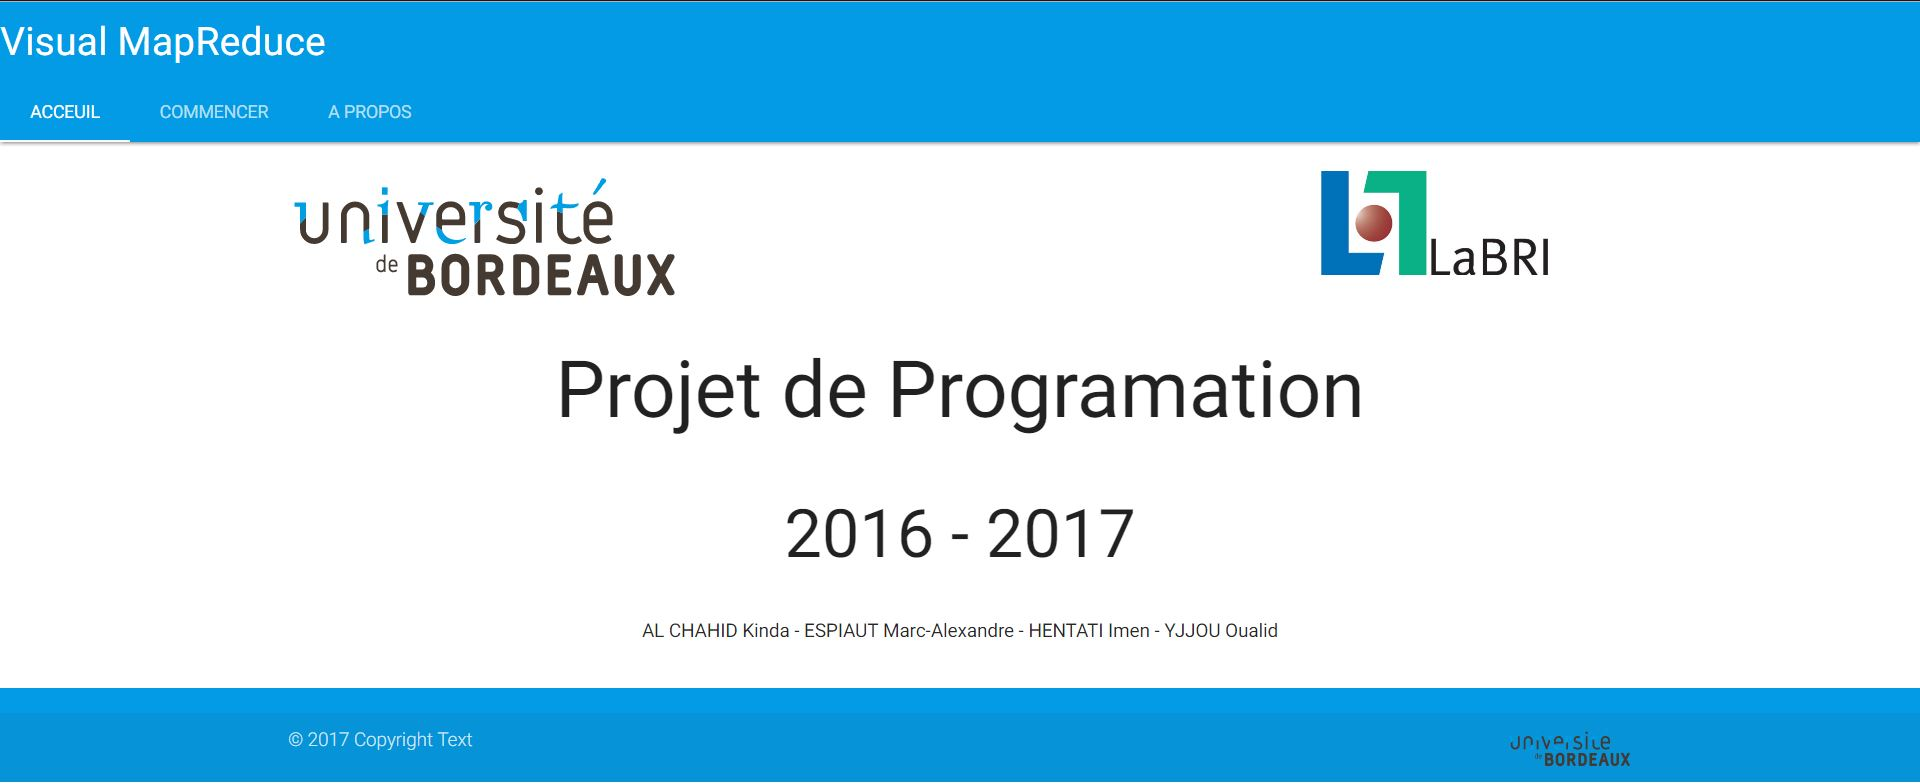
\includegraphics[width=1\textwidth]{images/resultat_acceuil.jpg}
        \caption{Page d'acceuil}
        \label{fig:PageAcceuil}
\end{figure}
\subsection{Page de simulation}
\begin{figure}[H]
  \centering
    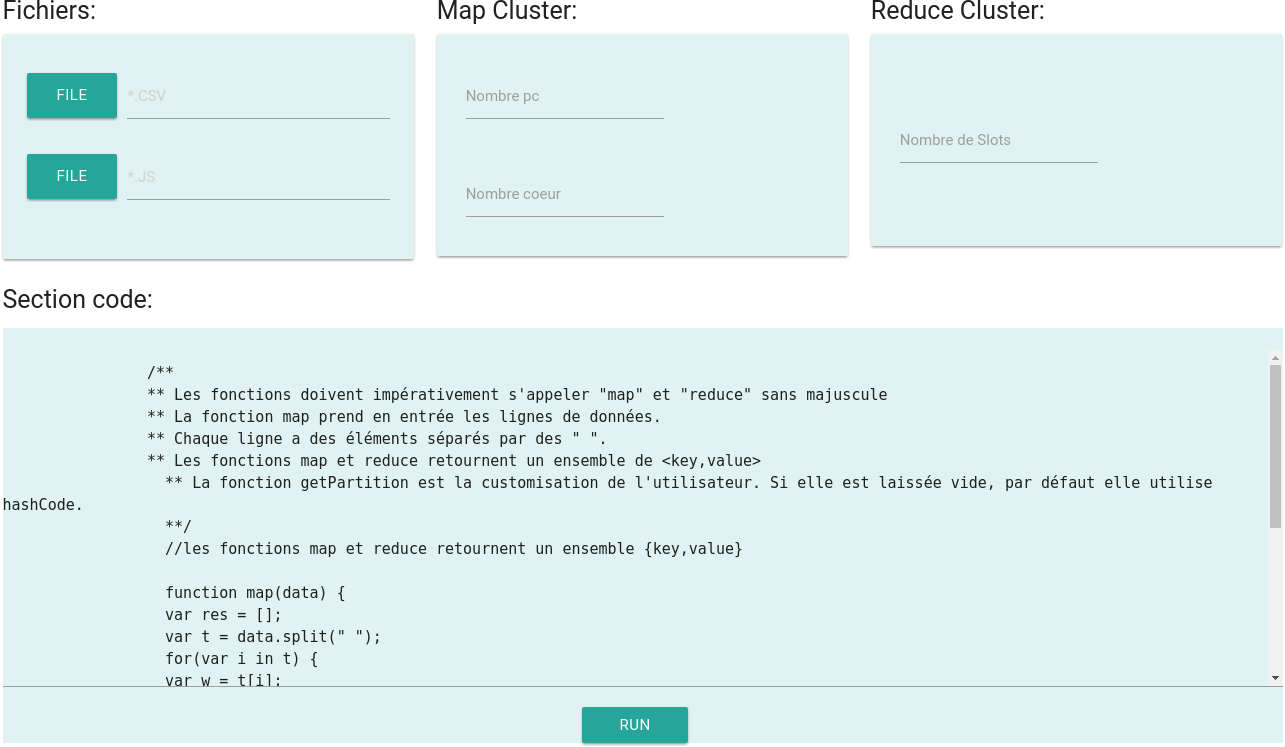
\includegraphics[width=1\textwidth]{images/resultat_simulation_1.jpg}
        \caption{Simulation - Paramètres}
        \label{fig:Sim-Param}
\end{figure}
\begin{figure}[H]
  \centering
    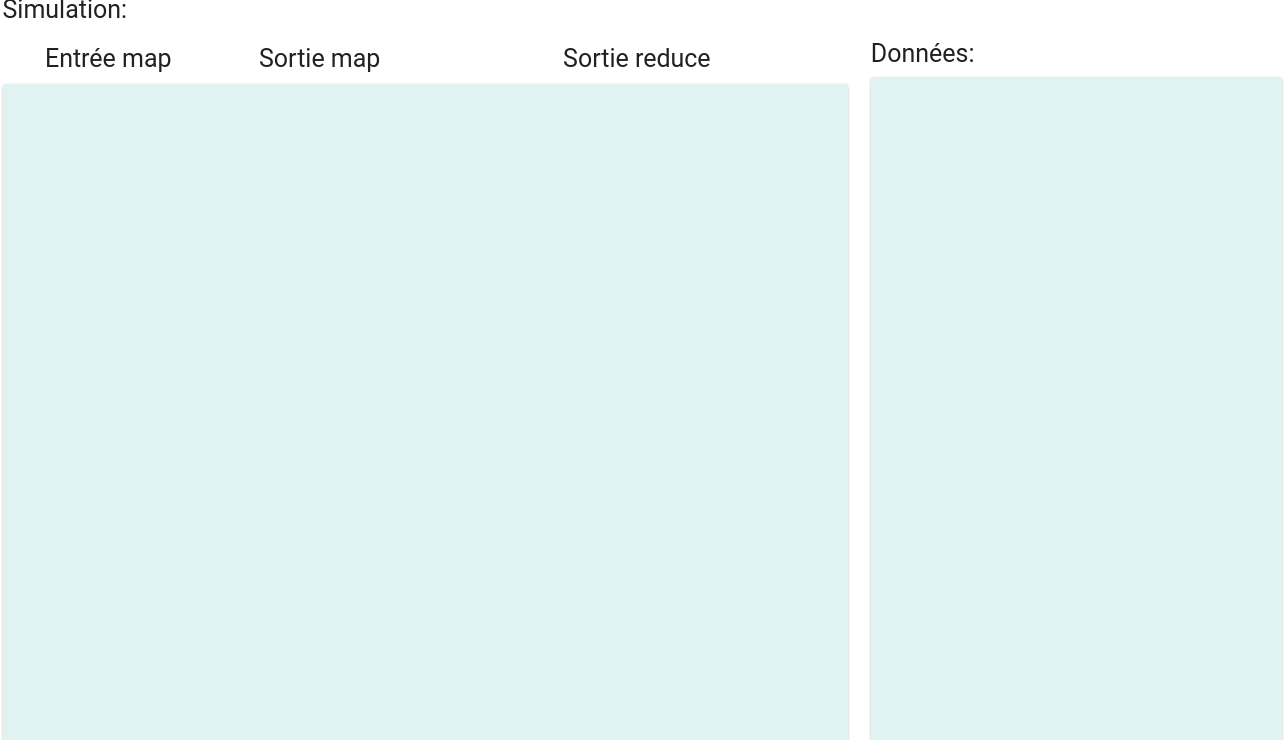
\includegraphics[width=1\textwidth]{images/resultat_simulation_2.jpg}
        \caption{Simulation - Cluster et données}
        \label{fig:sim-cluster}
\end{figure}

\subsection{Page "A propos"}
\begin{figure}[H]
  \centering
    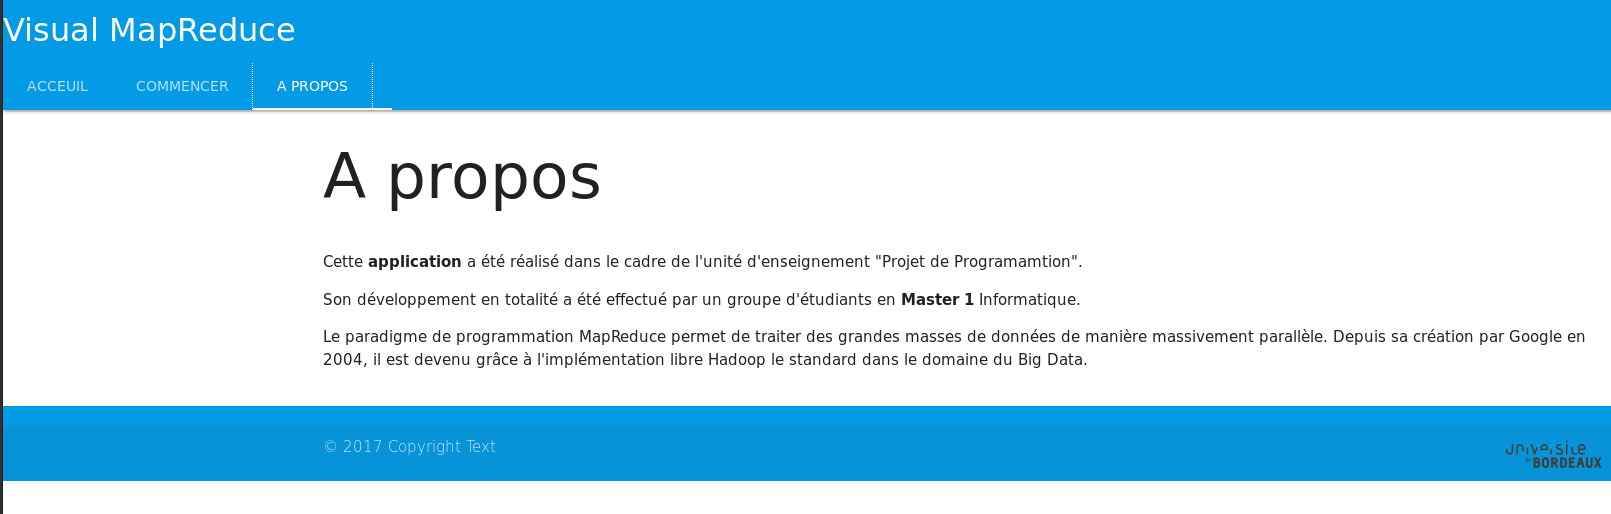
\includegraphics[width=1\textwidth]{images/apropos.png}
        \caption{Page "A propos"}
        \label{fig:Apropos}
\end{figure}
\section{Résultats de la simulation}
La simulation (Figure \ref{fig:Fatum}) est permise grâce à FATuM, ce bloc html est donc uniquement affiché par cette bibliothèque.
\begin{figure}[H]
  \centering
    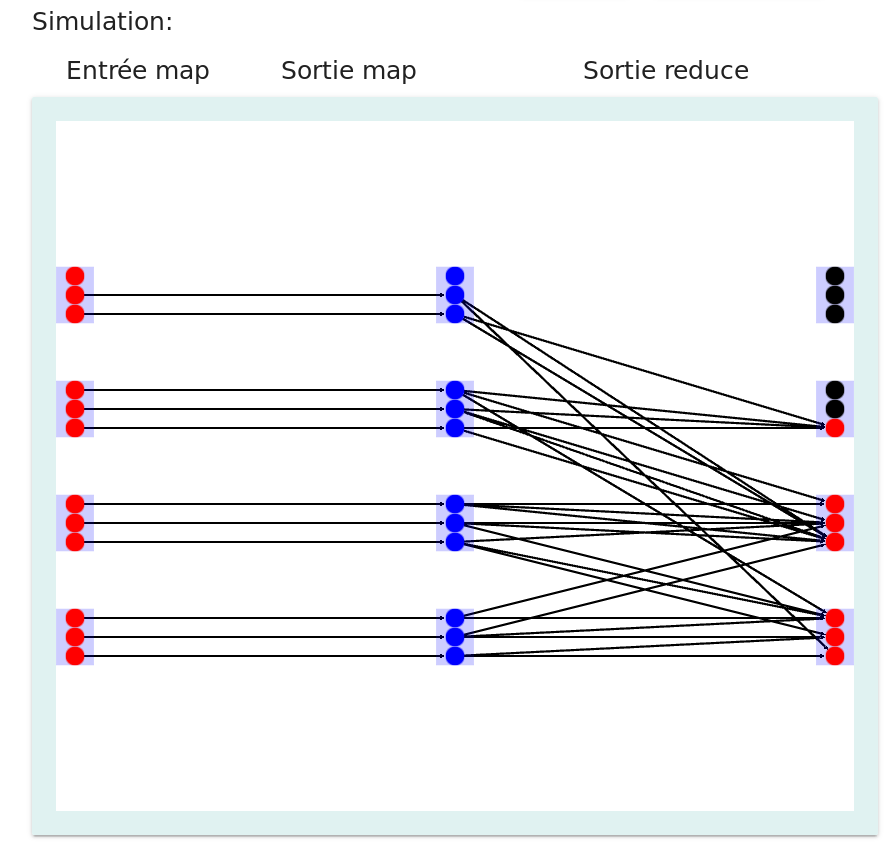
\includegraphics[width=0.75\textwidth]{images/simulation_pdp.png}
        \caption{FATuM}
        \label{fig:Fatum}
\end{figure}
\section{Résultats sur console}
Enfin, à la demande du client, nous avons mis les résultats des différentes étapes en sortie de console (Figure \ref{fig:SortieConsole}).
\begin{figure}[H]
  \centering
    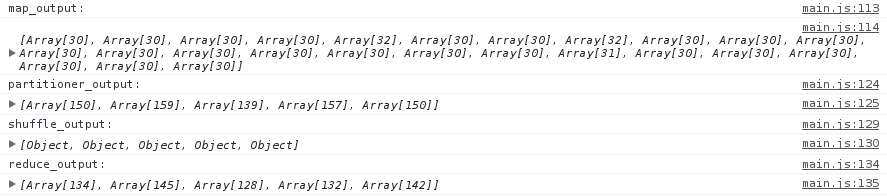
\includegraphics[width=1\textwidth]{images/resultat_console.png}
        \caption{Sortie Console}
        \label{fig:SortieConsole}
\end{figure}
